% Source-SHA256: 818fdb5deaa08233b61aa1c51d1184ec8d13fe6f5d029c85ca9be76c293e8dfd
% !TeX program = xelatex
\documentclass[a4paper,11pt]{article}
\usepackage{fontspec}
\IfFontExistsTF{TeX Gyre Pagella}{\setmainfont{TeX Gyre Pagella}}{\setmainfont{P052}}
\IfFontExistsTF{TeX Gyre Heros}{\setsansfont{TeX Gyre Heros}}{\setsansfont{Nimbus Sans}}
\IfFontExistsTF{TeX Gyre Cursor}{\setmonofont{TeX Gyre Cursor}[Scale=0.88]}{\setmonofont{Nimbus Mono PS}[Scale=0.88]}
\usepackage{babel}
\babelprovide[import,main]{spanish}
\usepackage{microtype}
\usepackage[a4paper,margin=2.4cm,headheight=23pt,headsep=10pt,footskip=1.1cm]{geometry}
\raggedbottom
\setlength{\emergencystretch}{3em}
\hyphenpenalty=10000
\exhyphenpenalty=10000
\clubpenalty=10000
\widowpenalty=10000
\usepackage{xcolor}
\definecolor{navybg}{HTML}{0B1D2E}
\definecolor{navydeep}{HTML}{123049}
\definecolor{lightblue}{HTML}{8FD3FE}
\definecolor{amber}{HTML}{F5A623}
\definecolor{softgray}{HTML}{5B6570}
\usepackage{titlesec,needspace}
\setcounter{secnumdepth}{-1}
\setcounter{tocdepth}{2}
\titleformat{\section}{\sffamily\Large\bfseries\color{navydeep}\raggedright}{}{0pt}{}
\titleformat{\subsection}{\sffamily\large\bfseries\color{navydeep}\raggedright}{}{0pt}{}
\titlespacing*{\section}{0pt}{20pt}{9pt}
\titlespacing*{\subsection}{0pt}{14pt}{6pt}
\usepackage{fancyhdr}
\pagestyle{fancy}
\fancyhf{}
\fancyhead[L]{\small\sffamily\color{softgray}Drop Route}
\fancyhead[R]{\small\sffamily\color{softgray}Manual de uso}
\fancyfoot[L]{\small\sffamily\color{softgray}Versión 1.0.1}
\fancyfoot[R]{\small\sffamily\color{softgray}\thepage}
\renewcommand{\headrulewidth}{0.4pt}
\usepackage{array,longtable,booktabs,calc}
\newcounter{none}
\renewcommand{\arraystretch}{1.15}
\usepackage{enumitem}
\setlist[itemize]{leftmargin=1.4em,itemsep=3pt,topsep=5pt}
\setlist[enumerate]{leftmargin=1.8em,itemsep=3pt,topsep=5pt}
\usepackage{fvextra,framed,seqsplit}
\fvset{fontsize=\small,breaklines=true,breakanywhere=true,frame=leftline,framerule=1.4pt,rulecolor=\color{lightblue},framesep=8pt}
\let\originaltexttt\texttt
\renewcommand{\texttt}[1]{\originaltexttt{\seqsplit{#1}}}
\providecommand{\tightlist}{\setlength{\itemsep}{2pt}\setlength{\parskip}{0pt}}
\usepackage{graphicx,xurl}
\usepackage[section]{placeins}
\usepackage{amssymb,newunicodechar}
\usepackage[colorlinks=true,linkcolor=navydeep,urlcolor=navydeep,pdftitle={Drop Route - Manual de uso},pdfauthor={Jesús Quevedo Rodríguez}]{hyperref}
\usepackage{bookmark}
\newunicodechar{♭}{\texorpdfstring{\ensuremath{\flat}}{\unichar{9837}}}
\newunicodechar{♯}{\texorpdfstring{\ensuremath{\sharp}}{\unichar{9839}}}
\newunicodechar{✓}{\texorpdfstring{\ensuremath{\checkmark}}{\unichar{10003}}}
\newunicodechar{✗}{\texorpdfstring{\ensuremath{\times}}{\unichar{10007}}}
\newunicodechar{→}{\texorpdfstring{\ensuremath{\rightarrow}}{\unichar{8594}}}
\newunicodechar{←}{\texorpdfstring{\ensuremath{\leftarrow}}{\unichar{8592}}}
\setlength{\parindent}{0pt}
\setlength{\parskip}{6pt}
\renewcommand{\topfraction}{0.95}
\renewcommand{\bottomfraction}{0.95}
\renewcommand{\textfraction}{0.05}
\renewcommand{\floatpagefraction}{0.6}
\setcounter{topnumber}{3}
\setcounter{totalnumber}{4}
\begin{document}
\begin{titlepage}
\newgeometry{margin=0cm}
\thispagestyle{empty}
\pagecolor{navybg}
\color{white}
\vspace*{3cm}
\begin{center}
{\sffamily\bfseries\fontsize{16}{19}\selectfont\color{amber} DROP ROUTE\par}
\vspace{1.4cm}
{\sffamily\bfseries\fontsize{30}{38}\selectfont Manual de uso\par}
\vspace{0.8cm}
{\sffamily\fontsize{14}{20}\selectfont\color{lightblue} Reconocer voicings y continuar rutas II--V--I\par}
\vfill
{\sffamily\small Autor del proyecto: Jesús Quevedo Rodríguez\par}
{\sffamily\small Versión 1.0.1\par}
{\sffamily\small Repositorio: a01653/Drop\_Route\par}
\vspace{2cm}
\end{center}
\nopagecolor
\end{titlepage}
\restoregeometry
\setcounter{page}{2}
\tableofcontents
\newpage
Autor: Jesús Quevedo Rodríguez. Versión 1.0.3.

Drop Route es un juego para estudiar voicings de guitarra y recorridos
II-V-I. Las preguntas trabajan en Do (C), sin audio; el modo estudio
permite transponer las formas. Guarda el progreso en el navegador del
dispositivo; no usa cuentas ni sincroniza datos.

\hypertarget{1-elegir-quuxe9-practicar}{%
\section{1. Elegir qué practicar}\label{1-elegir-quuxe9-practicar}}

Al abrir la aplicación aparece el menú. Puedes elegir \textbf{Reconocer
voicings}, \textbf{Rutas II-V-I} o \textbf{Modo estudio}.

En reconocimiento seleccionas Drop, set de cuerdas y dificultad. En
rutas se usa Drop 2 y eliges set, modo mayor o menor y tramo de la
secuencia. El modo estudio sirve para consultar formas y rutas sin
responder preguntas.

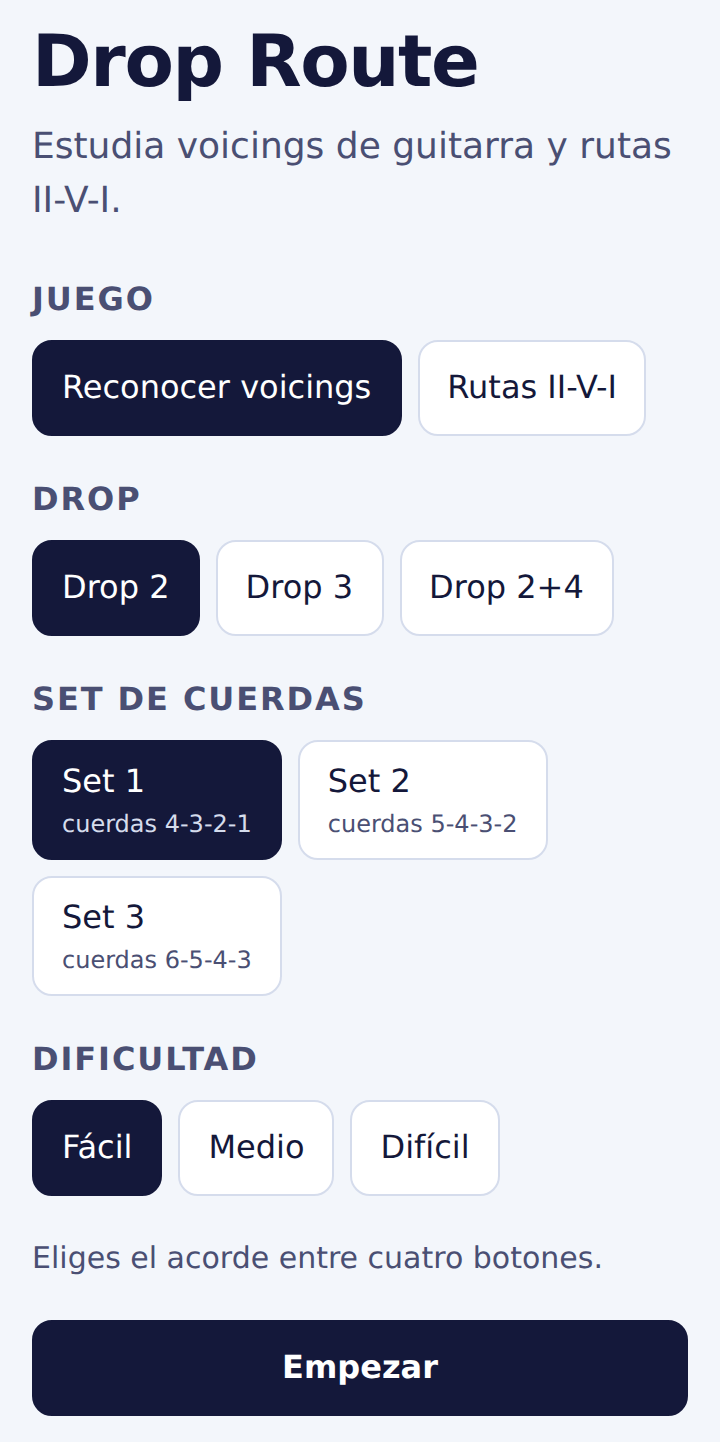
\includegraphics[width=0.48\linewidth,height=0.62\textheight,keepaspectratio]{../manuals/capturas/menu-reconocimiento-360.png}

\emph{Figura 1. Menú de reconocimiento.}

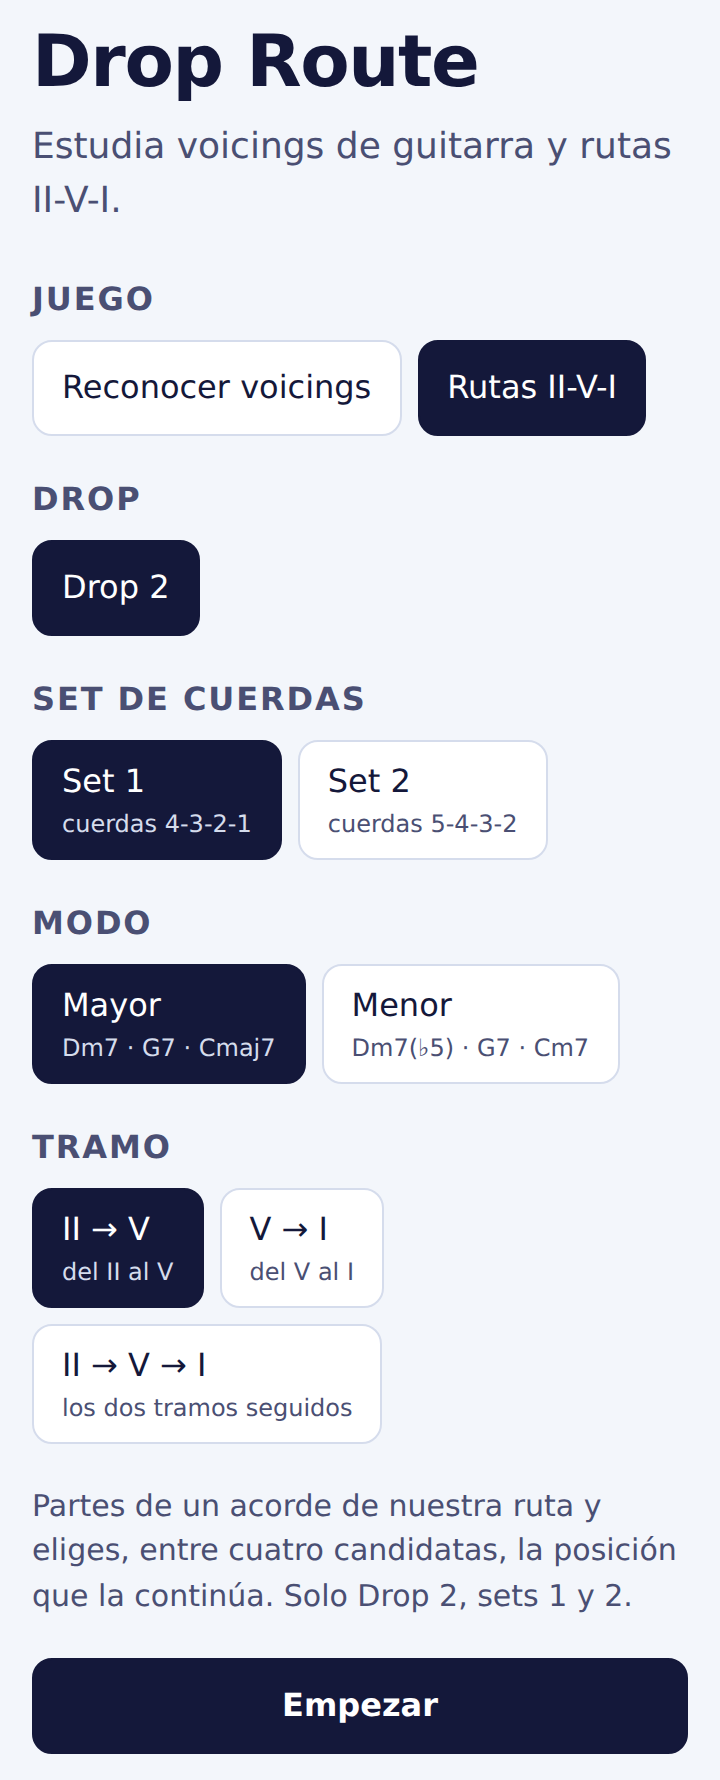
\includegraphics[width=0.48\linewidth,height=0.62\textheight,keepaspectratio]{../manuals/capturas/menu-rutas-360.png}

\emph{Figura 2. Menú de rutas II-V-I.}

\hypertarget{2-reconocer-voicings}{%
\section{2. Reconocer voicings}\label{2-reconocer-voicings}}

Cada pregunta muestra una tarjeta neutra: ves la posición física de las
notas, pero no el nombre del acorde ni los grados de la solución.

\hypertarget{fuxe1cil}{%
\subsection{Fácil}\label{fuxe1cil}}

Elige entre Cmaj7 / C6, C7, Cm7 y Cm7(b5). El orden cambia entre
preguntas. La opción mayor agrupa las formas con séptima y con sexta;
siempre tiene el mismo nombre para no dar pistas. Cuando la plantilla
usa C6, se pregunta esa posición con sexta y, al corregir, la séptima
original aparece en gris como referencia. Las formas mantienen cuatro
voces activas.

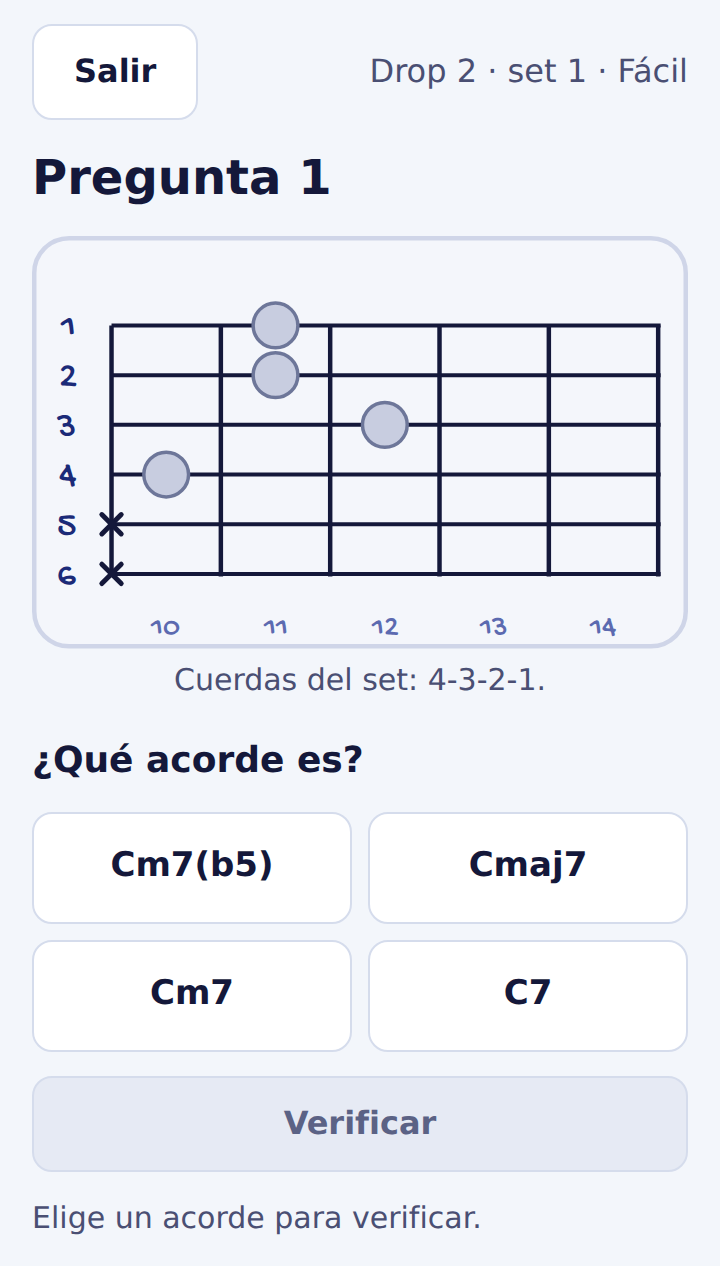
\includegraphics[width=0.48\linewidth,height=0.62\textheight,keepaspectratio]{../manuals/capturas/facil-pregunta-360.png}

\emph{Figura 3. Nivel fácil antes de verificar.}

Al verificar, la respuesta se bloquea. Si fallas, el acorde elegido se
marca y la solución queda identificada también con texto y símbolos.

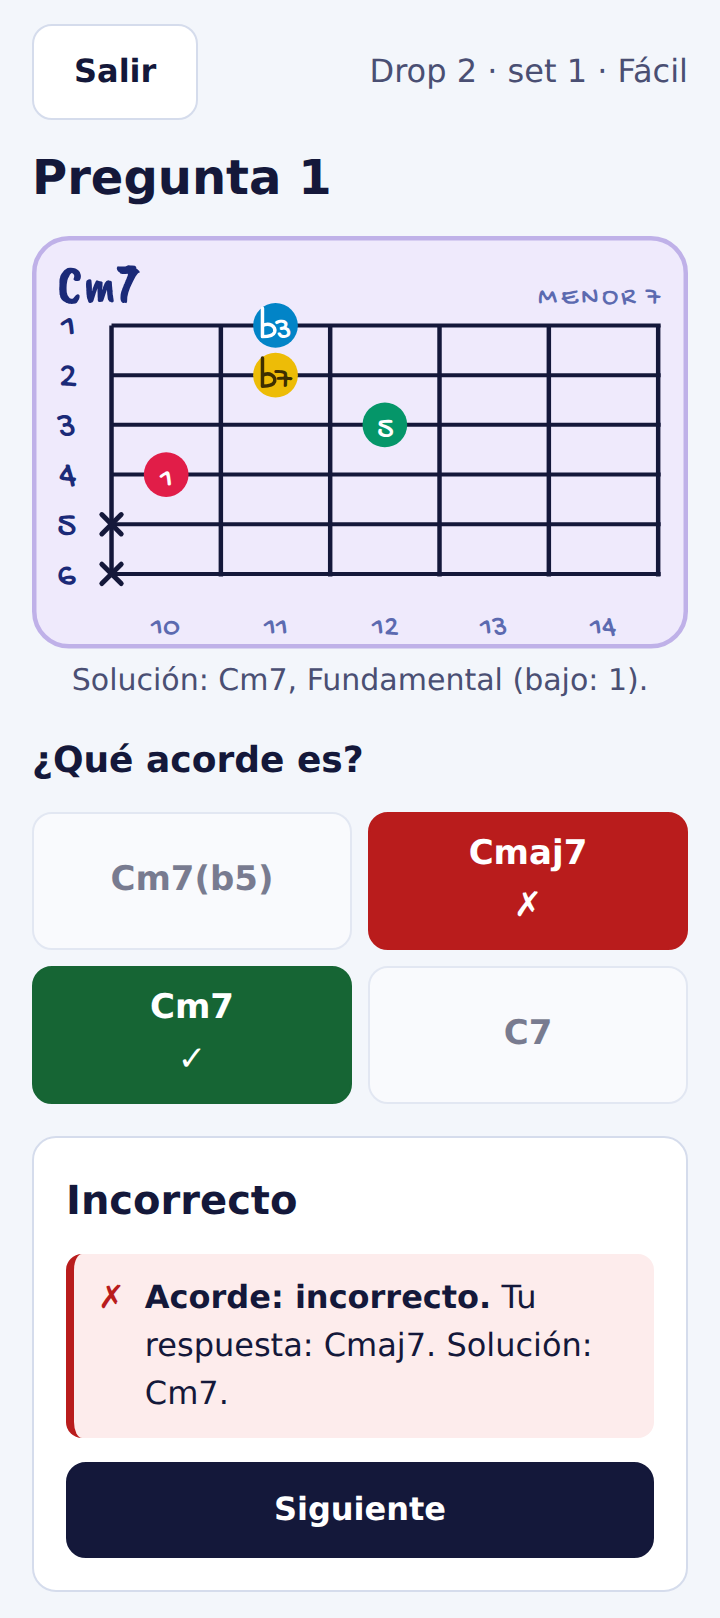
\includegraphics[width=0.48\linewidth,height=0.62\textheight,keepaspectratio]{../manuals/capturas/facil-correccion-360.png}

\emph{Figura 4. Corrección del nivel fácil.}

\hypertarget{medio}{%
\subsection{Medio}\label{medio}}

Indica el acorde y la inversión con los dos selectores. La aplicación
comprueba ambos campos por separado.

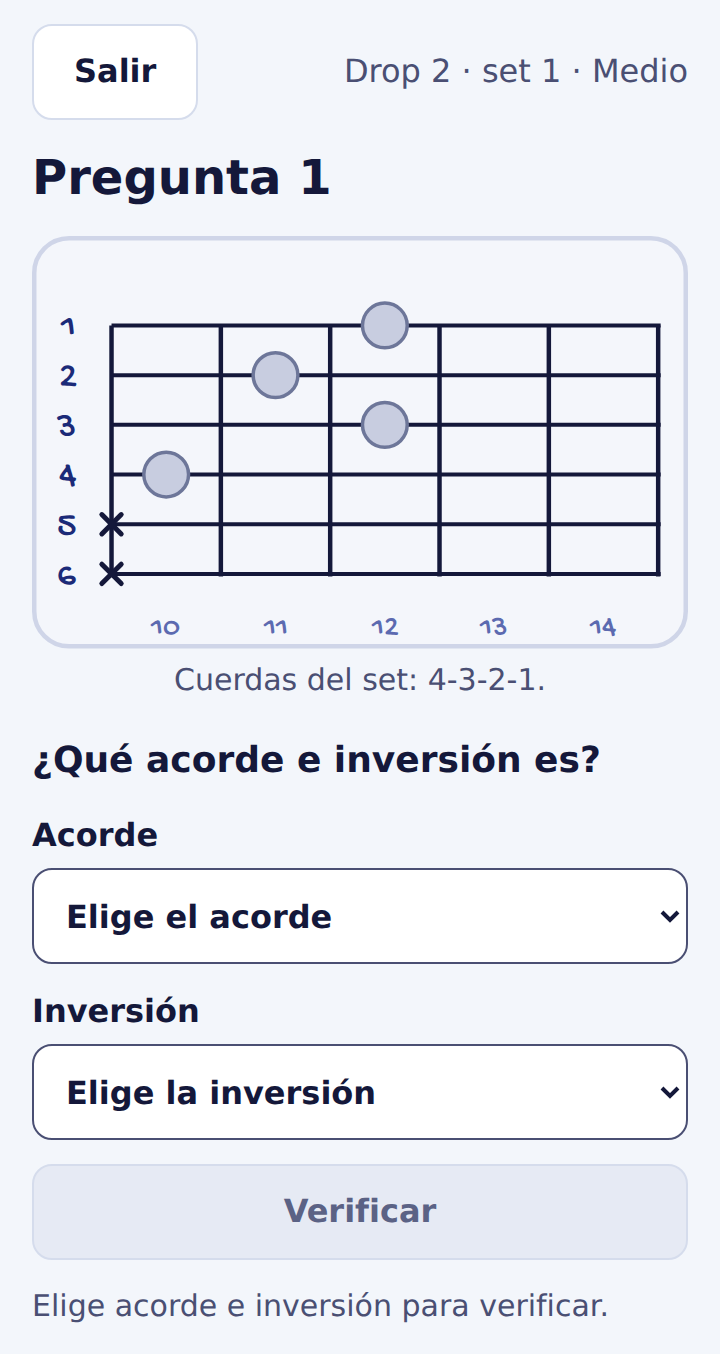
\includegraphics[width=0.48\linewidth,height=0.62\textheight,keepaspectratio]{../manuals/capturas/medio-pregunta-360.png}

\emph{Figura 5. Nivel medio antes de verificar.}

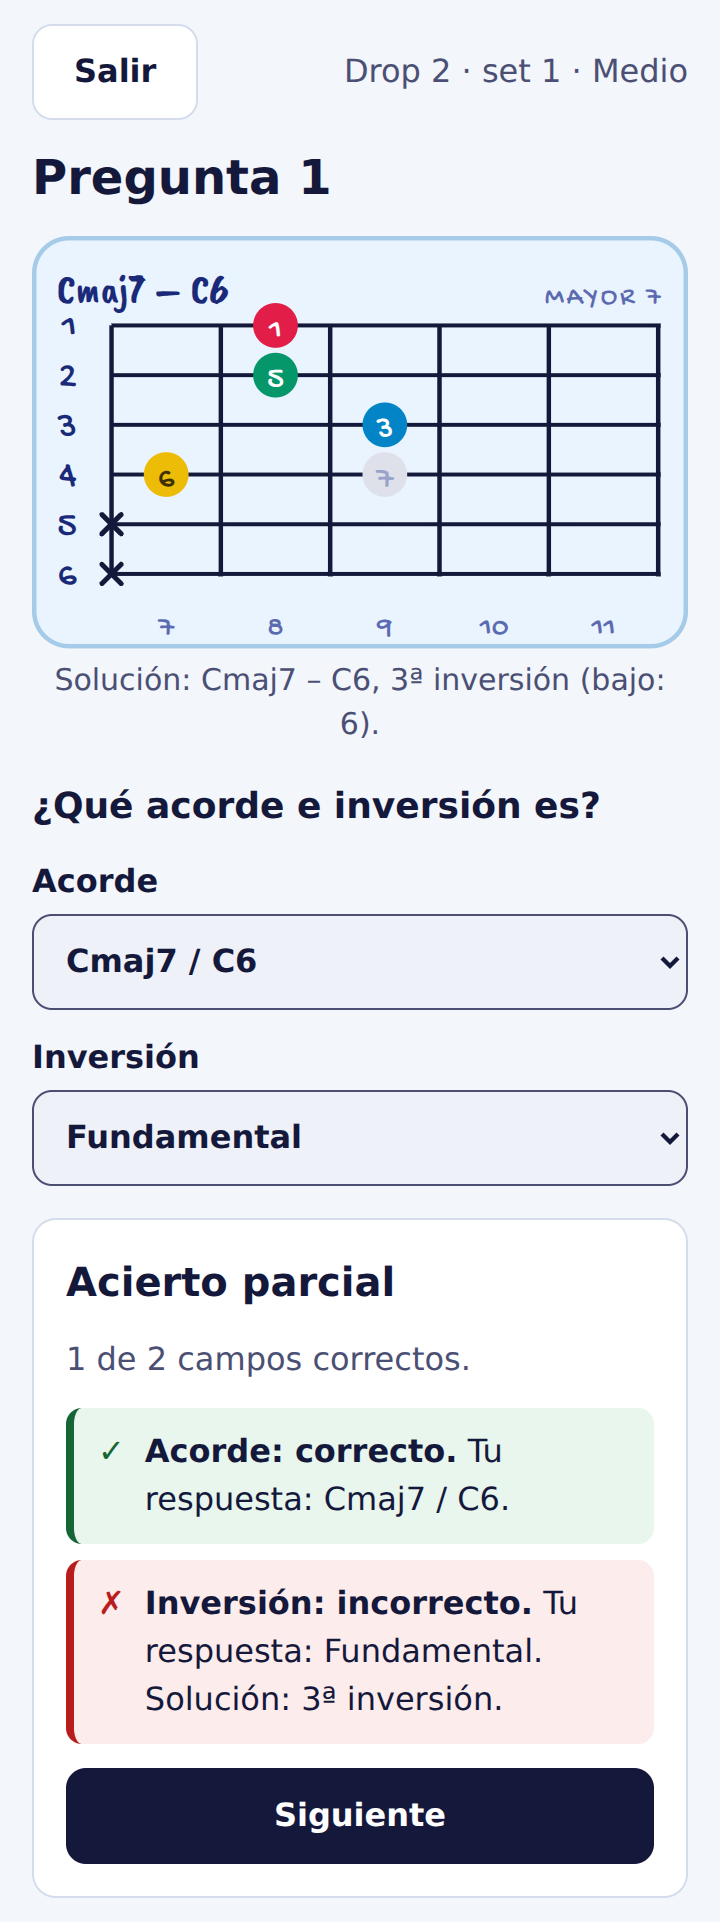
\includegraphics[width=0.48\linewidth,height=0.62\textheight,keepaspectratio]{../manuals/capturas/medio-correccion-360.png}

\emph{Figura 6. Corrección campo por campo.}

\hypertarget{difuxedcil}{%
\subsection{Difícil}\label{difuxedcil}}

Además del acorde y la inversión, coloca los cuatro grados sobre los
círculos de la tarjeta. El banco incluye siempre 1, 3, ♭3, 5, ♭5, 6, 7 y
♭7. En las variantes con sexta se coloca 6, no 7, en su círculo. Puedes
arrastrar, usar dos toques, teclado o los controles de colocación sin
arrastre.

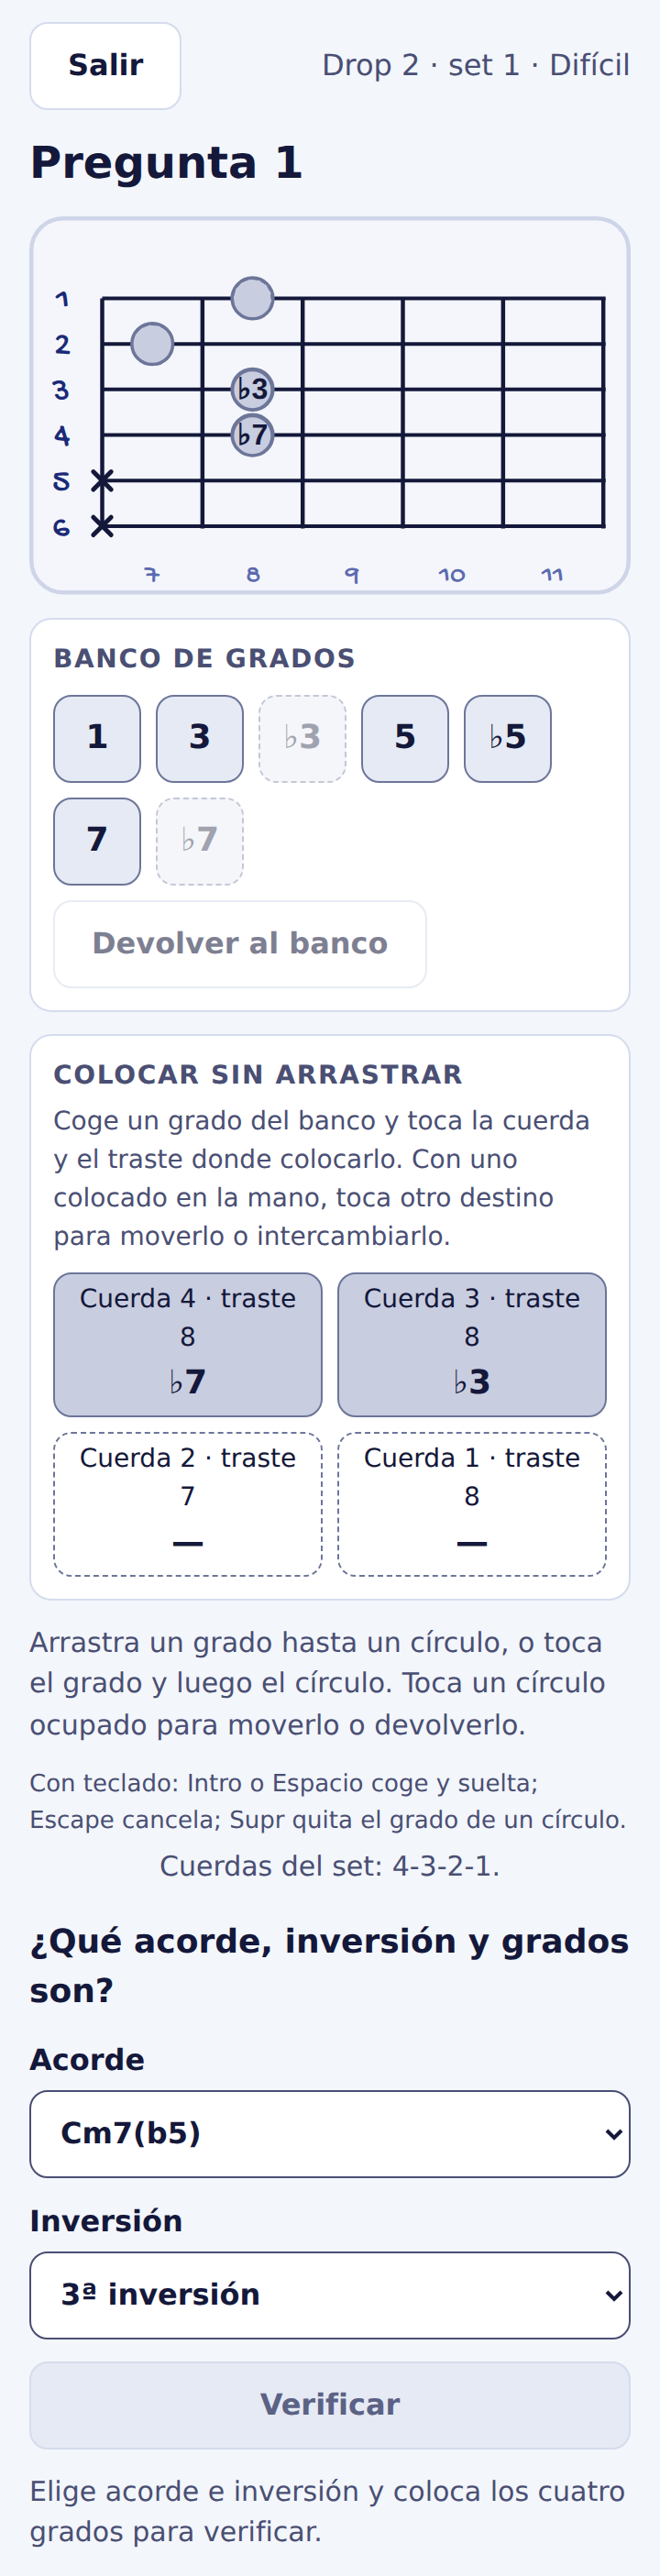
\includegraphics[width=0.48\linewidth,height=0.62\textheight,keepaspectratio]{../manuals/capturas/dificil-pregunta-360.png}

\emph{Figura 7. Nivel difícil durante la respuesta.}

La corrección compara acorde, inversión y cada círculo. Solo cuenta como
acierto completo cuando todos los campos son correctos.

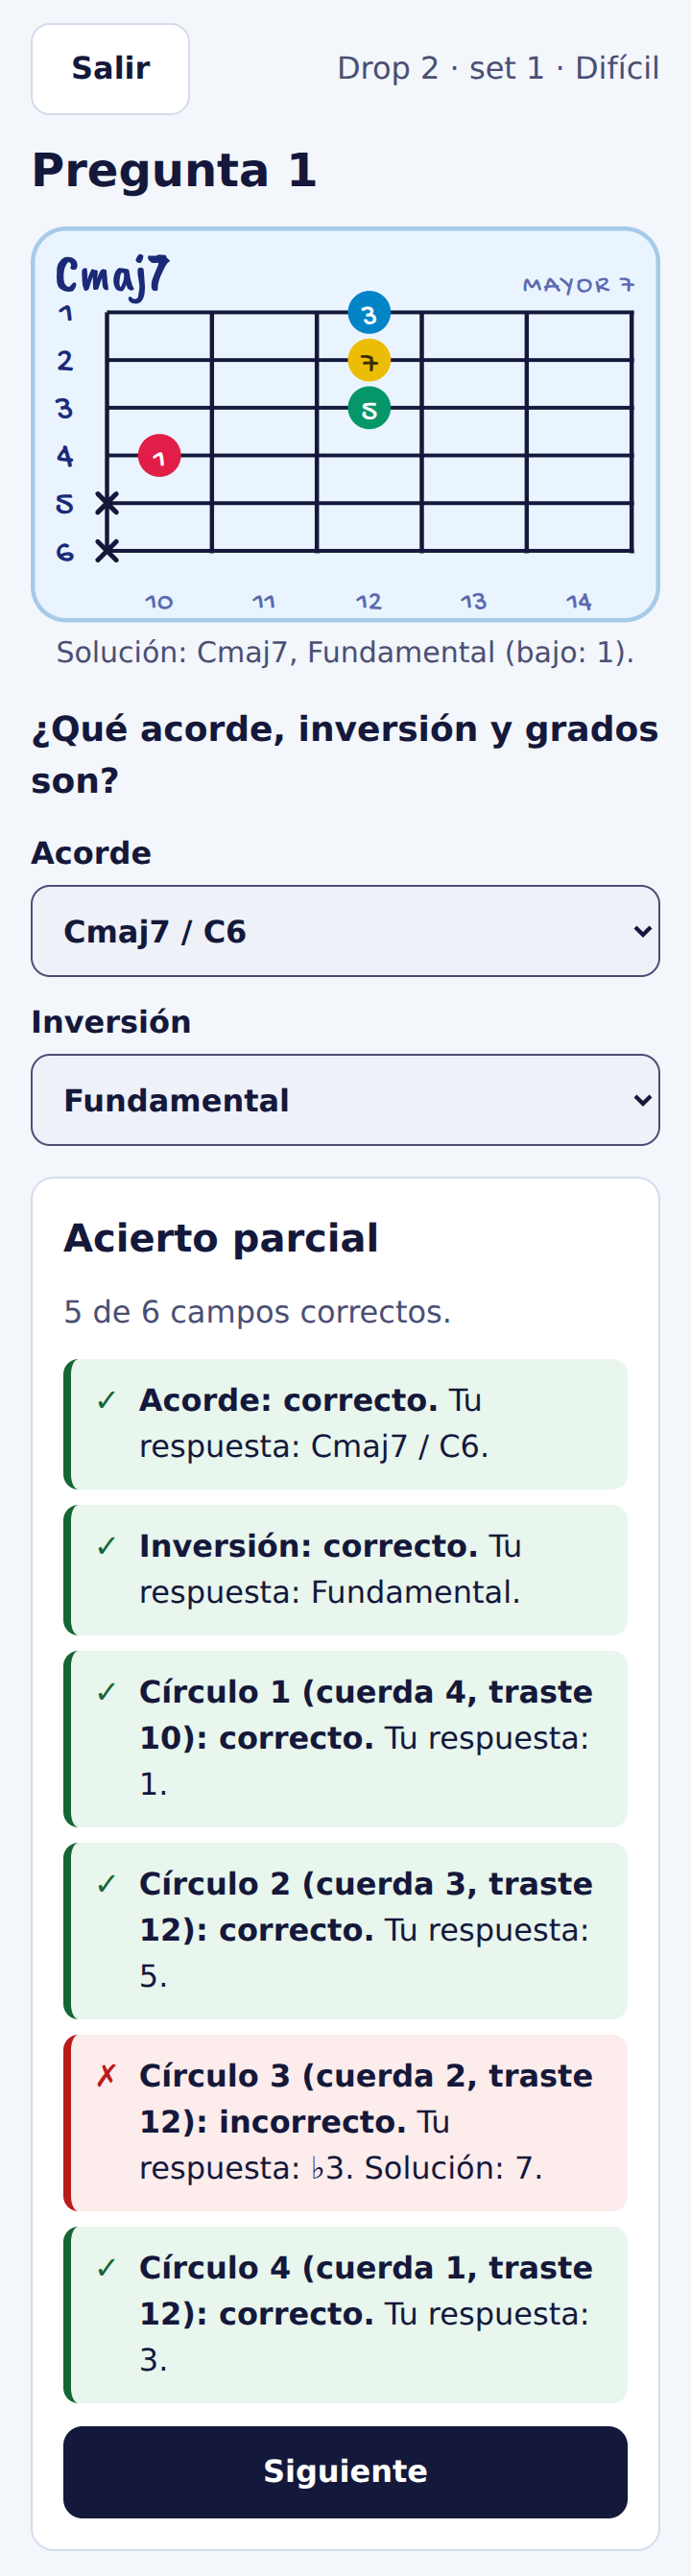
\includegraphics[width=0.48\linewidth,height=0.62\textheight,keepaspectratio]{../manuals/capturas/dificil-correccion-360.png}

\emph{Figura 8. Corrección del nivel difícil.}

\hypertarget{3-rutas-ii-v-i}{%
\section{3. Rutas II-V-I}\label{3-rutas-ii-v-i}}

Las rutas disponibles son:

\begin{itemize}
\tightlist
\item
  Mayor: Dm7 → G7 → Cmaj7.
\item
  Menor: Dm7(♭5) → G7 → Cm7.
\end{itemize}

Elige el tramo \textbf{II → V}, \textbf{V → I} o \textbf{II → V → I}. La
partida se mantiene visible y debajo aparece una candidata. Cambia entre
las cuatro posiciones con el selector 1-4, el gesto lateral o el
teclado.

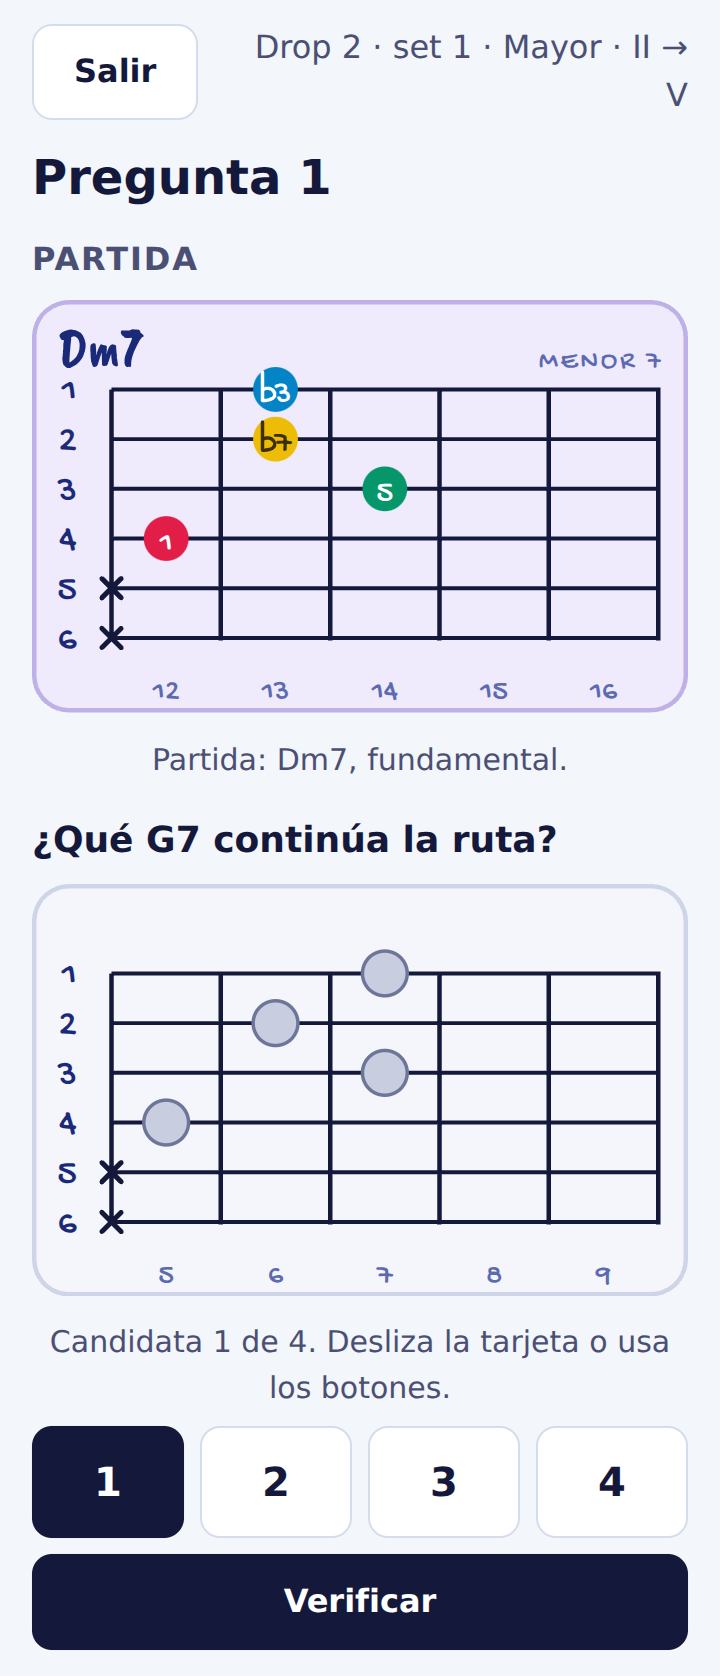
\includegraphics[width=0.48\linewidth,height=0.62\textheight,keepaspectratio]{../manuals/capturas/ruta-pregunta-360.png}

\emph{Figura 9. Partida, candidata y selector.}

La verificación indica si elegiste la posición usada por esa ruta. Otra
inversión del mismo acorde puede ser musicalmente válida y, aun así, no
ser la posición de la secuencia estudiada.

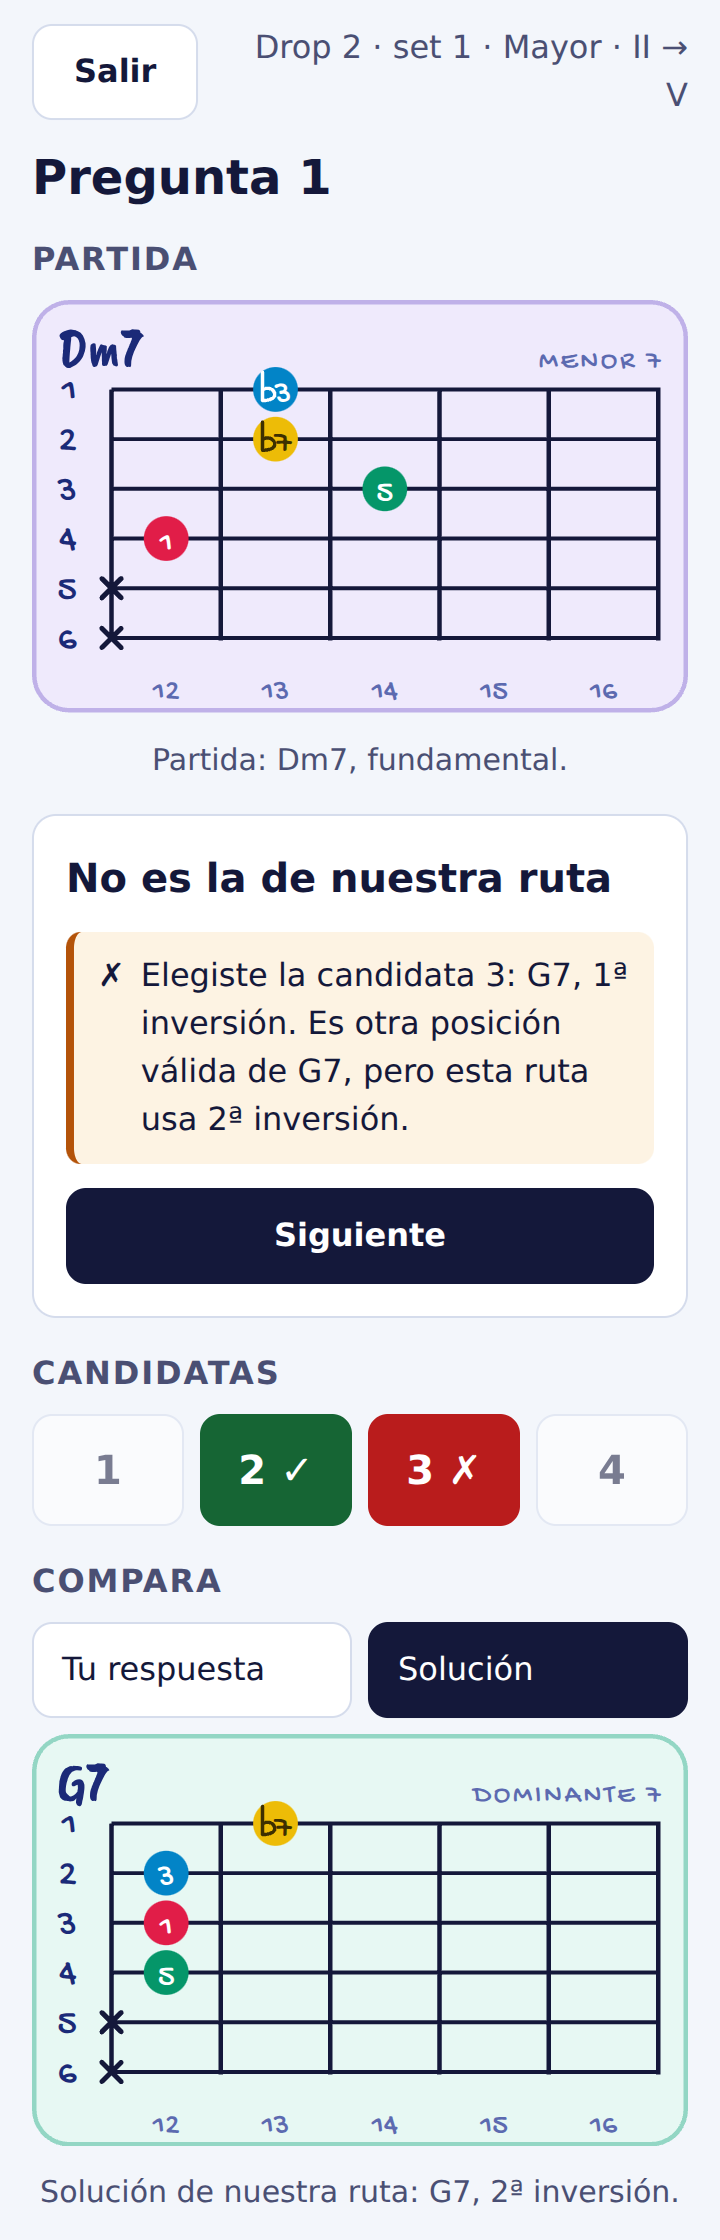
\includegraphics[width=0.48\linewidth,height=0.62\textheight,keepaspectratio]{../manuals/capturas/ruta-fallo-solucion-360.png}

\emph{Figura 10. Solución de la ruta.}

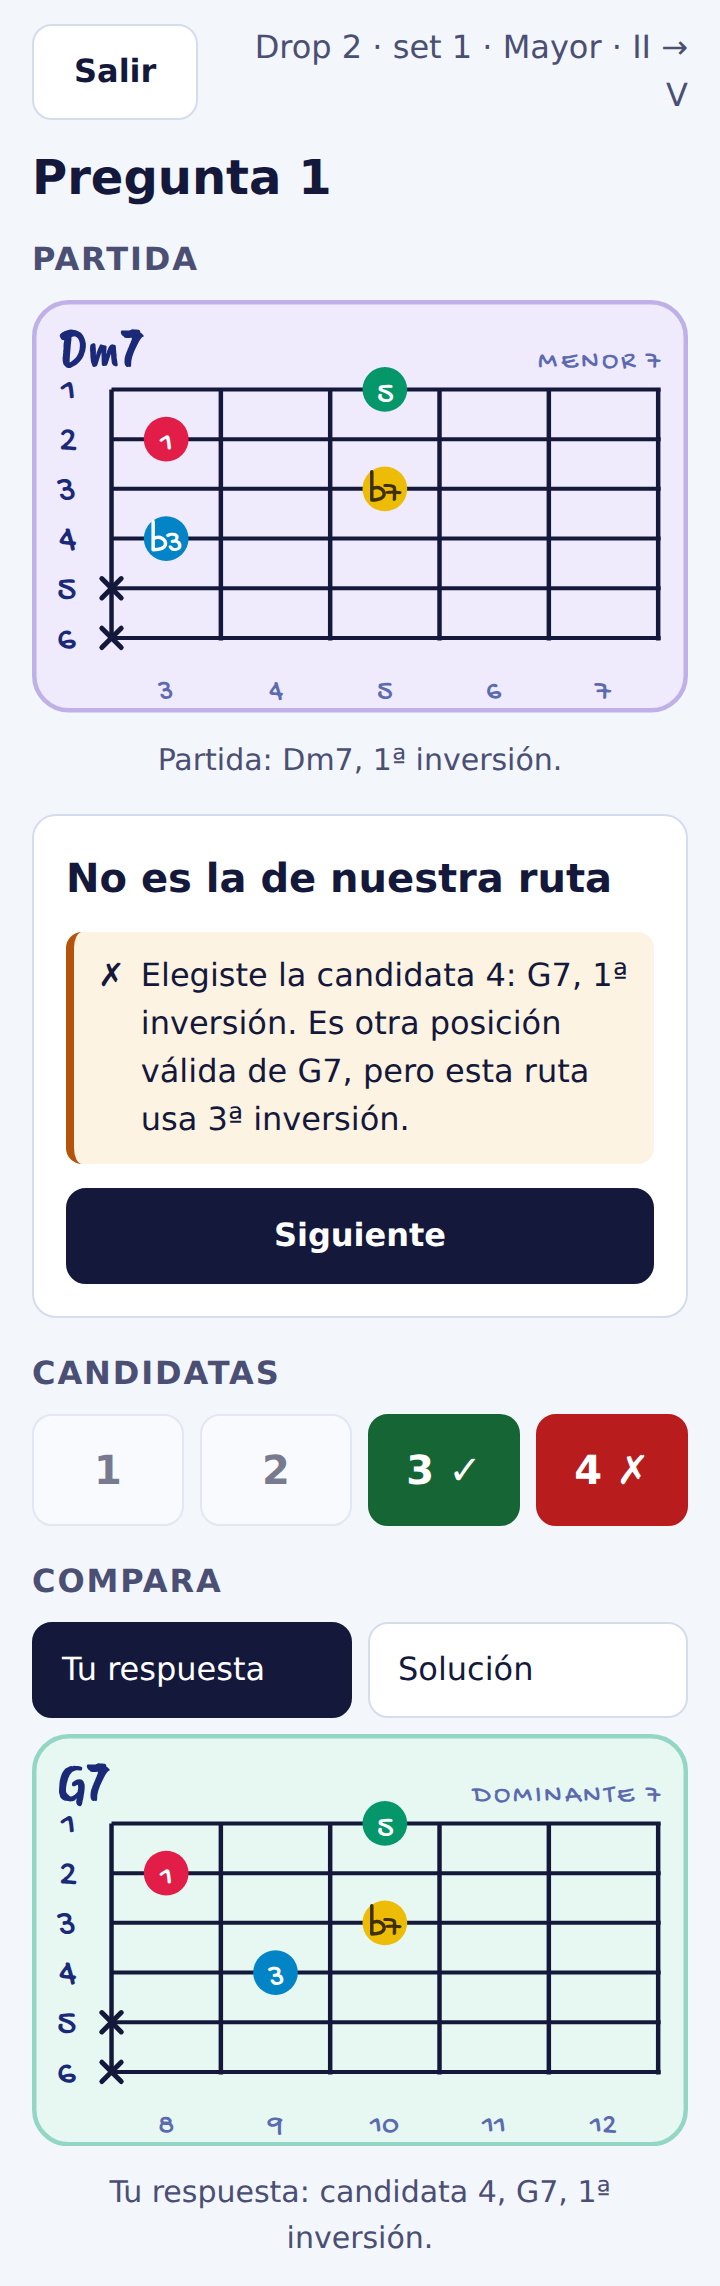
\includegraphics[width=0.48\linewidth,height=0.62\textheight,keepaspectratio]{../manuals/capturas/ruta-fallo-tu-respuesta-360.png}

\emph{Figura 11. Comparación con tu respuesta.}

\hypertarget{4-modo-estudio}{%
\section{4. Modo estudio}\label{4-modo-estudio}}

En el menú, abre \textbf{Modo estudio} y selecciona \textbf{Rutas
II-V-I}. Elige el set, el modo mayor o menor, la ruta y la tonalidad.
Verás los acordes II, V e I juntos y el movimiento de las voces.

La columna sombreada marca el traste donde cae la raíz del acorde II. Se
repite en las tres tarjetas y se desplaza al cambiar de tonalidad. El
número de ese traste aparece en negrita. El modo estudio no suma
intentos ni modifica el progreso.

\hypertarget{5-progreso}{%
\section{5. Progreso}\label{5-progreso}}

Cada pregunta suma un intento cuando pulsas \textbf{Verificar}. Salir,
cambiar una selección o mirar la corrección no añade intentos. El panel
del menú muestra intentos y aciertos por juego y configuración.

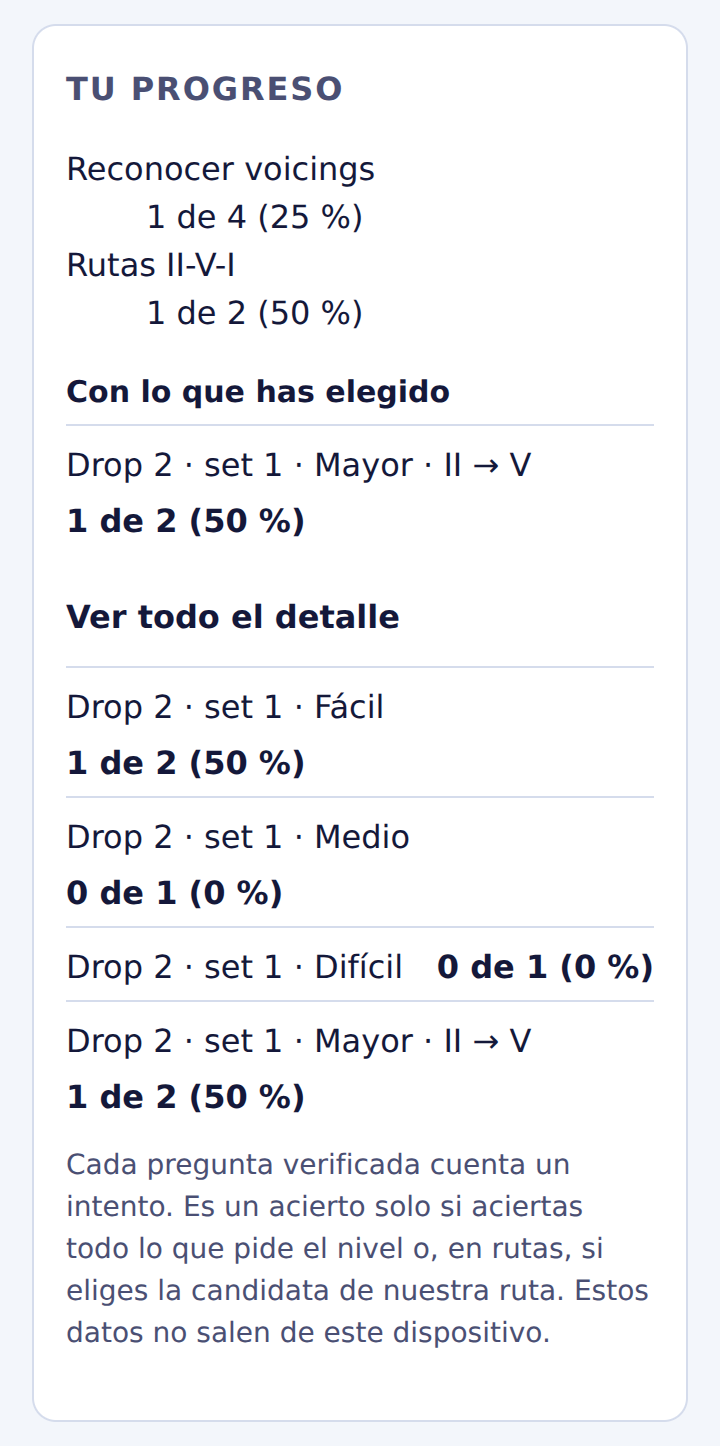
\includegraphics[width=0.48\linewidth,height=0.62\textheight,keepaspectratio]{../manuals/capturas/progreso-detalle-360.png}

\emph{Figura 12. Detalle del progreso local.}

Los datos quedan en este navegador y dispositivo. Si borras los datos
del sitio, se pierde ese progreso. Si el navegador no puede guardar,
Drop Route lo avisa y permite seguir jugando en memoria.

\hypertarget{6-actualizar-y-jugar-sin-conexiuxf3n}{%
\section{6. Actualizar y jugar sin
conexión}\label{6-actualizar-y-jugar-sin-conexiuxf3n}}

Después de una primera carga completa con conexión, la PWA guarda los
recursos de la aplicación para poder recargar y jugar sin red.

Cuando hay una versión nueva, el menú ofrece \textbf{Actualizar ahora}.
La versión nueva no se activa mientras tienes una pregunta abierta. Si
existen cambios que solo están en memoria, el aviso lo indica antes de
actualizar.

\hypertarget{7-luxedmites-de-esta-entrega}{%
\section{7. Límites de esta
entrega}\label{7-luxedmites-de-esta-entrega}}

No incluye audio, transposición en las respuestas, cuentas ni
sincronización. Tampoco ofrece notificaciones, sesiones adaptativas o
restauración del progreso. Las rutas se limitan a Drop 2 en los sets 1 y
2.
\end{document}
